\documentclass[a4paper,12pt,dvips]{thesis}
\usepackage[latin1]{inputenc}
\usepackage[italian]{babel}
\usepackage{amsfonts}
\usepackage{amssymb,amsmath}
\usepackage[pdftex]{graphicx}
\usepackage{latexsym}

\newtheorem{theorem}{Teorema}[section]
\newtheorem{lemma}{Lemma}[section]
\newtheorem{corollary}{Corollario}[section]
\newtheorem{remark}{Osservazione}[section]
\newtheorem{definition}{Definizione}[section]

\usepackage{amsmath}


%%%%%%%%%%%%%%%%%%%%%%%%%%%%%%%%%%%%%%%%%%%%%%%%%%%%%%%%%%%%%%%%%%%%%%%%%%%%%%%%%%%%%%%%%
% Macro algoritmi in un frame, con caption e label. Si usano cosi':



\newcommand{\algoritmo}{
\begin{figure}[htbp]%
\begin{center}%
\begin{framepage}{\textwidth}%
\singlespace\small%
\begin{tabbing}%
}

\newcommand{\finealgoritmo}[2]{
\end{tabbing}%
\end{framepage}%
\end{center}%
\caption{#2}%
\label{fi:#1}%
\end{figure}%
\noindent%
}

\newenvironment{chapterAbstract}
         {\singlespace \begin{quote}\begin{itshape}\begin{small}  \hugeinitial}
         {\newline \line(1,0){200} \end{small}\end{itshape}\end{quote} \onehalfspace}
                                           

\university{Firenze} \faculty{Ingegneria} \dept{Ingegneria dell'Informazione} \course{Ingegneria Informatica}
\accademicyear{2019 - 2020} 
\supervisor{Marco Bertini}
\supervisor{Secondo Supervisore}
\advisor{Correlatore 1}
\author{Andrea Moscatelli}
\title{Riconoscimento di azioni umane usando tecniche di apprendimento profondo per la stima della posa}

%%%%%%%%%%%%%%%%%%%%%%%%%%%%%%%%%%%%%%%%%%%%%%%%%%%%%%%%%%%%%%%%%%%%%%%%%%%%%%%%%%%%%%%%%

%\def\conclusionname{Conclusioni}
%\def\conclusion{
%  \chapter*{\conclusionname
%        %\@mkboth{\uppercase{\conclusionname}}{\uppercase{\conclusionname}}
%        }%
%  \addcontentsline{toc}{chapter}{\conclusionname}%
%}



\begin{document}
\sffamily
\maketitle

\onehalfspace
\oddsidemargin  1.75cm 
\evensidemargin 1.75cm
\hyphenation{words}

\tableofcontents

\newpage

%\algoritmo
%1. \= iscriviti ad Ingegneria \\
%2. \> finch\a'e non ti stufi o non finisci gli esami \\
%   \> 2.1. \= prova a dare l' esame $i$ \\
%   \> 2.2. \> se superi l'esame $i$ \\
%   \>      \> 2.2.1. \= $i=i+1$ \\
%3. \> prepara la tesi oppure fattela fare (CEPU) \\
%4. \> scrivila in \LaTeX :) \\
%5. \> laureati
%\finealgoritmo{laurea}{Algoritmo per conseguire la Laurea in Ingegneria}
%
%
% ora si puo' fare riferimento all' algoritmo con \ref{fi:laurea}.






%%%%%%%%%%%%%%%%%%%%%%%%%%%%%%%%%%%%%%%%%%%%%%%%%%%%%%%%%%%%%%%%%%%%%%%%%%%%%%%%%%%%%%%%%



\preface{
prefazione
}

\introduction{
Introduzione
}

%% Stima della Posa %%%%%%%%%%%%%%%%%%%%%%%%%%%%%%%%%%




\chapter{Stima della posa}
\begin{figure}[htbp]
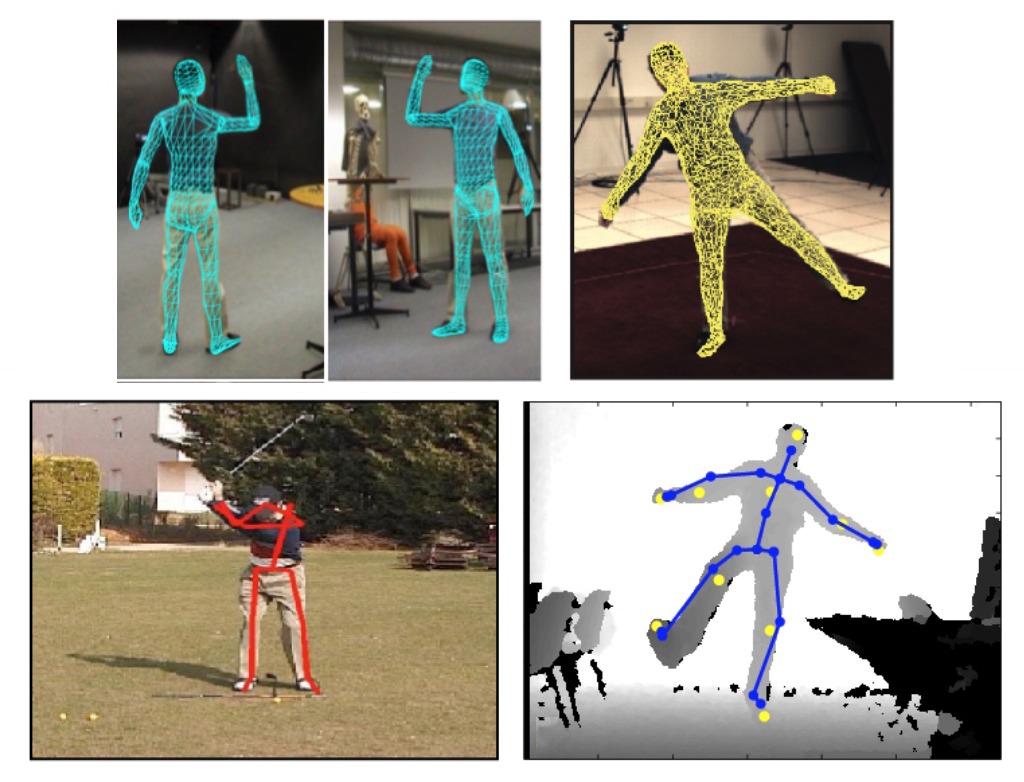
\includegraphics[width=\textwidth]{imgs/stimaPosaEsempi}
\caption{Esempi di stima della posa. In alto tre esempi di stima della posa utilizzando modelli di tipo volumetrico. In basso due esempi di stima della posa ottenuti utilizando modelli di tipo scheletrici. }
\end{figure}
\newpage
Cos � la stima della posa?\\
Quando parliamo di \textit{stima della posa} ci riferiamo ad una tecnica di \textit{computer vision} dedita al riconoscimento di figure umane all'interno di video ed immagini, cos� da poter riconosce ad esempio dove, all'interno dell'immagine, si trova la testa, il braccio, la gamba destra, etc.. del soggetto inquadrato. \\
Questa tecnica non va assolutamente confusa con tecniche di riconoscimento di persone, infatti la stima della posa � in grado solo di riconoscere dove le parti del corpo di un individuo sono situate all'interno dell'immagine, non \textit{chi} � inquadrato. \\

I campi di applicazione della stima della posa sono i pi� svariati: software interattivi che reagiscono al movimento della posa, robotica, realt� aumentata, animazione, fotoritocco intelligente, fitness, riabilitazione, etc. Stiamo parlando di un problema tutt'altro che semplice, infatti la condizione di luce dell'immagine, la variabilit� dell'ambiente circostante, l'inclinazione del soggetto inquadrato, rendono il riconoscimento della posa un problema non affatto banale. \\

Spinti dal crescente interesse, negli ultimi anni sono stati sviluppati diversi algoritmi per la stima della posa, raggiungendo in molti casi risultati davvero sorprendenti con un'accuratezza prossima alla perfezione. \\ 
\begin{figure}
\centering
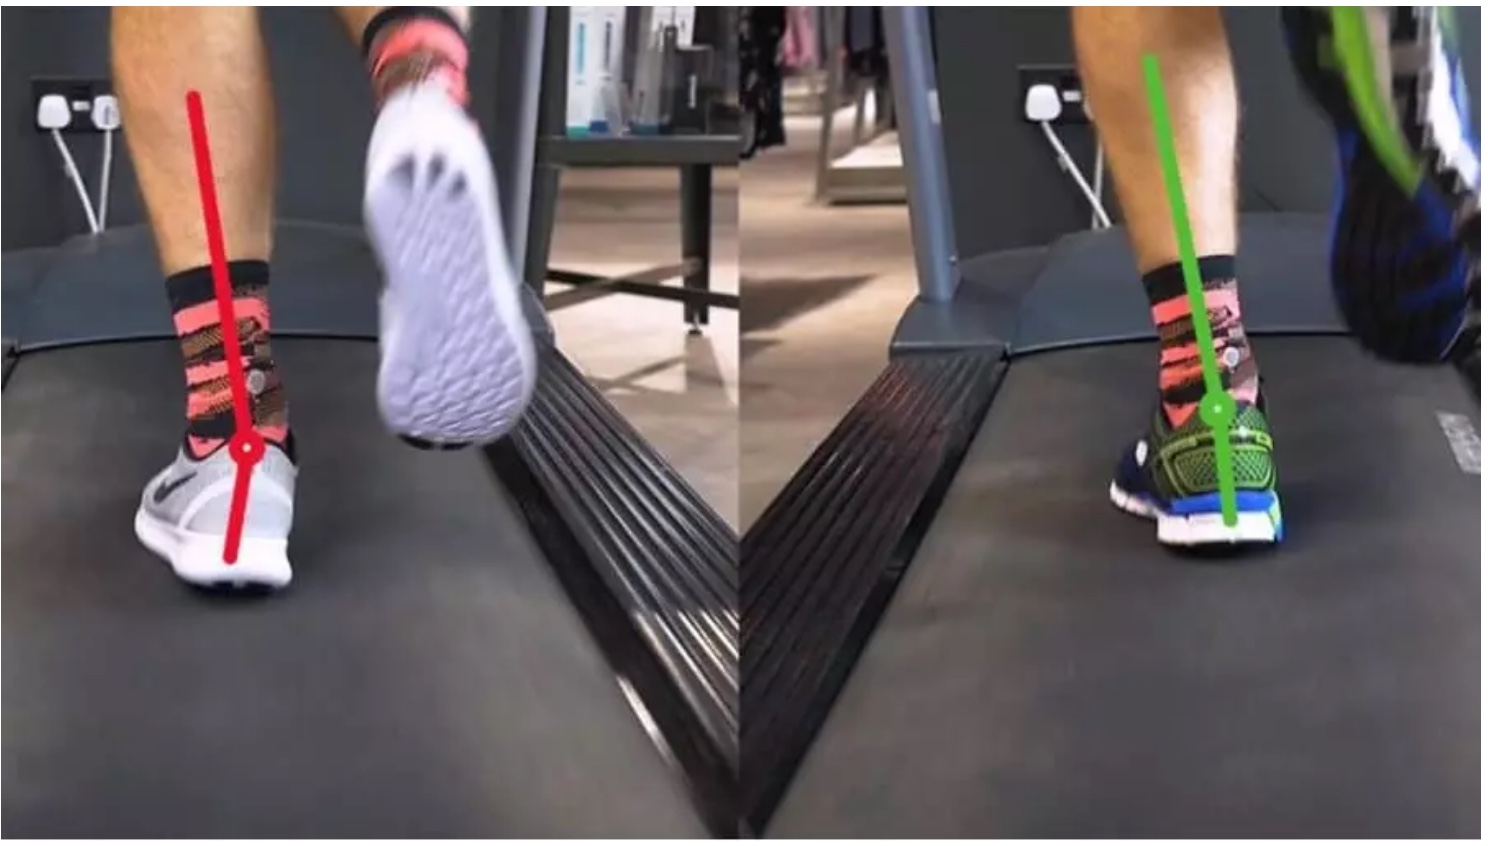
\includegraphics[width=0.7\textwidth]{imgs/stimaPosaEsempioFisio}
\caption{Un esempio di utilizzo in campo medico della stima della posa}
\end{figure}

La maggior parte dei software in circolazione in grado di stimare in maniera sufficientemente corretta la posa di un individuo non sono liberamente accessibili. Due fra i migliori algoritmi (ad oggi) di \emph{pose detection} sono sicuramente \textit{Posenet} \cite{PosenetArticle} e \textit{Detectron 2} \cite{Detectron2Link}, dei quali ci occuperemo in maniera pi� approfondita nei capitoli seguenti.


%% PoseNet %%%%%%%%%%%%%%%%%%%%%%%%%%%%%%%%%%
\chapter{PoseNet}
I recenti progressi nel campo della visione artificiale hanno permesso alla comunit� scientifica di spostarsi verso problemi ancora pi� articolati rispetto a quelli classici, come ad esempio il riconoscimento facciale, con l'obiettivo di riconoscere figure umane in contesti non vincolati e molto variabili. 

L'algoritmo \emph{PoseNet} � stato ideato proprio con lo scopo di identificare una o pi� figure umane in qualsiasi contesto, anche in contesti "affollati", ed essere in grado di identificare l'istanza di ogni persona stimandone i suoi \emph{punti chiave} (o \emph{key-points}).

Esistono due approcci principali per affrontare il rilevamento di pi� persone, la stima della posa e la segmentazione. L'approccio \emph{top-down} inizia identificando e localizzando approssimativamente le singole istanze di persona identificando il riquadro dell'immagine dentro le quali sono contenute, seguito da una fase di stima della posa o di separazione "primo piano-sfondo" nell'area identificata. Al contrario, l'approccio \emph{bottom-up} inizia localizzando entit� semantiche individuali, come ad esempio gambe, braccia, mani, etc, seguito dal loro raggruppamento in istanze di persone complete. PoseNet adotta questo secondo approccio.

In particolare PoseNet utilizza una rete neurale convoluzionale nella quale il costo computazionale del riconoscimento delle pose � essenzialmente indipendente dal numero di persone raffigurate nella scena ma dipende esclusivamente dalla scelta delle features della rete.

L'approccio adottato in PoseNet � quello di identificare dapprima tutti i punti chiave di ogni persona nell'immagine e successivamente raggrupparli in istanze utilizzando un processo "greedy", ovvero partendo dal rilevamento "pi� sicuro", e non come spesso accade da un punto fisso di riferimento (ad esempio il naso), avendo come vantaggio quello di funzionare bene anche se in disordine.

Oltre a stimare punti chiave sparsi, PoseNet stima anche maschere di segmentazione per ogni persona. Per fare ci�, viene allenata una seconda rete neurale con la quale viene associato ad ogni pixel $x_i$ dell'immagine la probabilit� di appartenenza di quel pixel ad ogni candidato $j$ identificato. Se la probabilit� � sufficientemente alta allora viene associato il pixel $x_i$ al candidato $j$.

Questo algoritmo � stato allenato utilizzando il dataset COCO \cite{COCO} che annota molte persone con 17 punti chiave (12 del corpo e 5 del volto), migliorando l'\emph{AP} (average-precision) dal precedente miglior risultato da 0,655 a 0,687. 

Questo metodo essendo molto semplice � anche quindi molto rapido, poich� non richiede alcuna fase supplementare di raffinamento dei risultati con tecniche di tipo \emph{box-based} o \emph{clustering}, facendo di PoseNet uno degli algoritmi pi� facilmente installabili su rete mobile.

\section{Stima dei key-points}
L'obiettivo di questa fase � quello di rilevare, in modo indipendente dall'istanza, tutti i key-points visibili appartenenti a qualsiasi persona dell'immagine. A tale scopo vengono prodotte delle \emph{heatmaps}, ovvero dei canali della rete neurale dediti al riconoscimento di particolari caratteristiche dell'immagine (una canale per ogni key-point) e degli \emph{offset} (due canali per ogni key-point per gli spostamenti in orizzontale e verticale). Sia $x_i$ la posizione 2-D nell'immagine, dove $i = 1, ... ,N$ e $N$ � il numero di pixels; $D_R (y) = \{ x:  \|x - y \| \leq R\}$ un disco di raggio $R$ centrato in $y$ e $y_{j,k}$ la posizione 2-D del $k$-esimo key-point della j-esima istanza di persona, con $j = 1, ..., M$, dove $M$ � il numero di istanze nell'immagine. 

Per ogni tipo di key-point $k = 1, ..., K$, viene impostato un task di classificazione binaria come segue. Viene generata una heatmap $p_k(x)$ tale che $p_k(x) = 1$ se $x \in D_R (y_{j,k})$ per qualsiasi istanza $j$, altrimenti $p_k(x) = 0$. Abbiamo quindi $K$ tasks di classificazione binaria indipendenti, una per ogni tipo di key-point. Ciascuno equivale a prevedere un disco di raggio $R$ attorno a un tipo di key-point specifico di qualsiasi persona nell'immagine.

Oltre alle heatmaps, vengono anche usati vettori di offset a \emph{corto raggio} $S_k(x)$ il cui scopo � quello di migliorare l'accuratezza della localizzazione dei key-points. Per ogni punto $x$ all'interno dei dischi ricavati al passo precedente, il vettore di offset 2-D a corto raggio $S_k(x) = y_{j,k} - x$ rappresenta la distanza fra il punto $x$ e il $k$-esimo key-point della $j$-esima persona. Vengono cosi generati $K$ vettori per ogni punto $x$ all'interno del disco definito che, combinati insieme, miglioreranno l'accuratezza della posizione predetta per ogni key-point. 

\section{Raggruppamento dei key-points in istanze di persona}

A questo � necessario per� capire come associare ogni key-point stimato ad ogni persona nell'immagine (nel caso ce ne sia pi� di una). 


%% Detecron 2 %%%%%%%%%%%%%%%%%%%%%%%%%%%%%%%%%%
\chapter{Detectron2}
Descrizione di cos� Detectron2



\chapter{Classificazione}
\section{Struttura della rete}
\section{Tecniche}

\subsection{Semplice}
\subsection{Tecnica dei centri}
\subsection{Tecnica delle differenze}

\chapter{Risultati ottenuti}

\chapter{Conclusioni}

\chapter{Sviluppi futuri}

%\thebibliography{}

\begin{thebibliography}{100}  % 100 is a random guess of the total number of references

\bibitem{PosenetArticle} \emph{"PersonLab: Person Pose Estimation and Instance Segmentation with a Bottom-Up, Part-Based, Geometric Embedding Model"} - George Papandreou, Tyler Zhu, Liang-Chieh Chen, Spyros Gidaris, Jonathan Tompson, Kevin Murphy - 2018
\bibitem{COCO}    Lin, T.Y., Cui, Y., Patterson, G., Ronchi, M.R., Bourdev, L., Girshick, R., Dollr,P. -  Coco 2016 keypoint challenge. - 2016
\bibitem{PosenetLink} PoseNet with TensorFlow.js - \emph{https://medium.com/tensorflow/real-time-human-pose-estimation-in-the-browser-with-tensorflow-js-7dd0bc881cd5}

\bibitem{Detectron2Link} Detectron2 - \emph{https://research.fb.com/wp-content/uploads/2019/12/4.-detectron2.pdf}
\end{thebibliography}




\end{document}